% !TeX spellcheck = en_GB
% !TeX program = lualatex
%
% v 2.3  Feb 2019   Volker RW Schaa
%		# changes in the collaboration therefore updated file "jacow-collaboration.tex"
%		# all References with DOIs have their period/full stop before the DOI (after pp. or year)
%		# in the author/affiliation block all ZIP codes in square brackets removed as it was not %         understood as optional parameter and ZIP codes had bin put in brackets
%       # References to the current IPAC are changed to "IPAC'19, Melbourne, Australia"
%       # font for ‘url’ style changed to ‘newtxtt’ as it is easier to distinguish "O" and "0"
%
\documentclass[a4paper,
               %boxit,        % check whether paper is inside correct margins
               %titlepage,    % separate title page
               %refpage       % separate references
               %biblatex,     % biblatex is used
               %keeplastbox,   % flushend option: not to un-indent last line in References
               %nospread,     % flushend option: do not fill with whitespace to balance columns
               %hyphens,      % allow \url to hyphenate at "-" (hyphens)
               %xetex,        % use XeLaTeX to process the file
               %luatex,       % use LuaLaTeX to process the file
               ]{jacow}
%
% ONLY FOR \footnote in table/tabular
%
\usepackage{pdfpages,multirow,ragged2e} %
\usepackage[spanish]{babel}

%
% CHANGE SEQUENCE OF GRAPHICS EXTENSION TO BE EMBEDDED
% ----------------------------------------------------
% test for XeTeX where the sequence is by default eps-> pdf, jpg, png, pdf, ...
%    and the JACoW template provides JACpic2v3.eps and JACpic2v3.jpg which
%    might generates errors, therefore PNG and JPG first
%
\makeatletter%
	\ifboolexpr{bool{xetex}}
	 {\renewcommand{\Gin@extensions}{.pdf,%
	                    .png,.jpg,.bmp,.pict,.tif,.psd,.mac,.sga,.tga,.gif,%
	                    .eps,.ps,%
	                    }}{}
\makeatother

% CHECK FOR XeTeX/LuaTeX BEFORE DEFINING AN INPUT ENCODING
% --------------------------------------------------------
%   utf8  is default for XeTeX/LuaTeX
%   utf8  in LaTeX only realises a small portion of codes
%
\ifboolexpr{bool{xetex} or bool{luatex}} % test for XeTeX/LuaTeX
 {}                                      % input encoding is utf8 by default
 {\usepackage[utf8]{inputenc}}           % switch to utf8

\usepackage[spanish]{babel}
%\usepackage[spanish]{babel}
\newenvironment{keywords}
{\par\small\textbf{Keywords}}
{\par}
%
% if BibLaTeX is used
%
\ifboolexpr{bool{jacowbiblatex}}%
 {%
  \addbibresource{jacow-test.bib}
  \addbibresource{biblatex-examples.bib}
 }{}
\listfiles

%%
%%   Lengths for the spaces in the title
%%   \setlength\titleblockstartskip{..}  %before title, default 3pt
%%   \setlength\titleblockmiddleskip{..} %between title + author, default 1em
%%   \setlength\titleblockendskip{..}    %afterauthor, default 1em

\begin{document}

\title{Learning Enriched Features for Fast Image Restoration and Enhancement}

\author{Fredy A. Huanca T.\thanks{Universidad Nacional San Agustín de Arequipa, fhuancat@unsa.edu.pe},
		Jose E. Perez M.\thanks{Universidad Nacional San Agustín de Arequipa, jperezma@unsa.edu.pe} y
		Henrry I. Arias M.\thanks{Universidad Nacional San Agustín de Arequipa, hariasm@unsa.edu.pe}}
	
\maketitle

%
\begin{abstract}
Image restoration is an important task in surveillance, computational photography, medical imaging, and remote sensing. Recently, convolutional neural networks (CNNs) have achieved dramatic improvements over conventional approaches. This paper presents a novel architecture with the collective goals of maintaining spatially precise high-resolution representations and receiving contextual solid information from the low-resolution representations. The core of the approach is a multi-scale residual block containing several key elements: parallel multi-resolution convolution streams, information exchange across the multi-resolution streams, spatial and channel attention mechanisms, and attention-based multi-scale feature aggregation. Extensive experiments on real image benchmark datasets demonstrate that MIRNet achieves state-of-the-art results for various image processing tasks.
\end{abstract}

\begin{keywords}
Image denoising, super-resolution, and image enhancement
\end{keywords}

\section{Introducción}

La restauración de imágenes es una tarea desafiante debido a la presencia de degradaciones en las imágenes adquiridas desde varios dispositivos. Las cámaras con capacidades limitadas, como las cámaras de los teléfonos inteligentes, a menudo producen imágenes ruidosas y de bajo contraste. Además, las condiciones de iluminación inadecuadas pueden dar como resultado imágenes demasiado oscuras o demasiado brillantes. El objetivo de la restauración de imágenes es recuperar la imagen limpia original de sus medidas corruptas, lo cual es un problema inverso mal planteado con múltiples soluciones posibles.

Los modelos de aprendizaje profundo han logrado avances significativos en la restauración y mejora de imágenes mediante el aprendizaje de antecedentes sólidos de conjuntos de datos a gran escala. Las redes neuronales convolucionales (CNN) existentes para la restauración de imágenes suelen seguir una arquitectura de codificador-decodificador o un enfoque de procesamiento de características de alta resolución (escala única). Los modelos de codificador-decodificador reducen progresivamente la resolución espacial de la imagen de entrada y luego la vuelven a mapear a la resolución original. Si bien estos modelos capturan un contexto amplio, a menudo pierden detalles espaciales finos, lo que dificulta su recuperación. Por otro lado, las redes de alta resolución conservan detalles espacialmente precisos pero tienen una capacidad limitada para codificar información contextual debido a su pequeño campo receptivo.

Para abordar estos desafíos, los autores proponen un nuevo enfoque multiescala llamado MIRNet. Este enfoque mantiene características de alta resolución en toda la jerarquía de la red, lo que minimiza la pérdida de detalles espaciales precisos. Emplea flujos de convolución paralelos para capturar contexto de múltiples escalas, lo que complementa la rama principal de alta resolución y proporciona representaciones de características más precisas y enriquecidas contextualmente. A diferencia de los enfoques multiescala existentes que procesan cada escala de forma independiente e intercambian información solo de arriba hacia abajo, MIRNet fusiona información en todas las escalas en cada nivel de resolución, lo que permite el intercambio de información de arriba hacia abajo y de abajo hacia arriba. Se utiliza un mecanismo de fusión de kernel selectivo para seleccionar dinámicamente kernels útiles de cada representación de rama, conservando sus características complementarias distintivas.

Nuestras principales contribuciones a este articulo incluyen lo siguiente:

\begin{itemize}[label=-]
  \item Un nuevo modelo de extracción de características que obtiene un conjunto complementario de características a través de múltiples escalas espaciales mientras mantiene las características originales de alta resolución para preservar detalles espaciales precisos.
  \item Un mecanismo repetido regularmente para el intercambio de información, donde las características a través de las ramas de resolución múltiple se fusionan progresivamente para mejorar el aprendizaje de la representación.
  \item Un nuevo enfoque para fusionar características de múltiples escalas utilizando una red de kernel selectiva que combina dinámicamente campos receptivos variables y conserva fielmente la información de la característica original en cada resolución espacial.
  \item Un diseño residual recursivo que descompone progresivamente la señal de entrada para simplificar el proceso de aprendizaje general y permite la construcción de redes muy profundas.
  \item Se realizan experimentos completos en cinco conjuntos de datos de referencia de imágenes reales para diferentes tareas de procesamiento de imágenes, incluida la eliminación de ruido de imágenes, la superresolución y la mejora de imágenes. Nuestro método logra resultados de última generación en los cinco conjuntos de datos. Además, evaluamos exhaustivamente nuestro enfoque para los desafíos prácticos, como la capacidad de generalización entre conjuntos de datos.
\end{itemize}
\section{Trabajo Relacionados}
 los autores revisan los métodos más relevantes para el procesamiento de imágenes de bajo nivel, incluyendo la eliminación de ruido, la superresolución y la mejora de imagen. A continuación, se resumen algunos de los métodos mencionados:
\begin{itemize}[label=-]
    \item Para la eliminación de ruido, como los basados en transformaciones de coeficientes y promedio de píxeles vecinos \cite{zhang2017beyond}. Además, se han propuesto enfoques basados en redes neuronales convolucionales profundas para esta tarea, como DnCNN \cite{zhang2017beyond} y RED30 \cite{mao2019red30}. Estos métodos utilizan arquitecturas profundas para aprender a eliminar el ruido de las imágenes a partir del conjunto de entrenamiento y generar imágenes limpias a partir de nuevas imágenes o imágenes dañadas por el ruido. Los resultados experimentales muestran que estos métodos pueden superar a los métodos clásicos en términos tanto visuales como cuantitativos.
    \item Para la superresolución, algunos de los métodos mencionados son bicubic interpolation, que es el método más comúnmente utilizado para generar imágenes de alta resolución a partir de imágenes de baja resolución, y enfoques basados en redes neuronales convolucionales profundas como VDSR \cite{vdsr}, DRCN \cite{kim2016deeply} y SRCNN \cite{dong2016image}. Estos métodos utilizan arquitecturas profundas para aprender a generar imágenes de alta resolución a partir del conjunto de entrenamiento y mejorar la calidad visual y cuantitativa de las imágenes generadas. Los resultados experimentales muestran que estos métodos pueden superar a los métodos clásicos como bicubic interpolation en términos tanto visuales como cuantitativos.
    \item Para la mejora de imagen,  algunos de los métodos mencionados son MemNet \cite{tai2017memnet} y FFDNet \cite{zhang2018ffdnet}, que son enfoques basados en redes neuronales convolucionales profundas que procesan características a su resolución original y fusionan información contextual de múltiples ramas paralelas. Además, se menciona el conjunto de datos MIT-Adobe FiveK \cite{dabov2007image}, que contiene imágenes de diversas escenas interiores y exteriores capturadas con cámaras DSLR en diferentes condiciones de iluminación, y se han utilizado las imágenes mejoradas por expertos como referencia para evaluar el rendimiento de los algoritmos. Los resultados experimentales muestran que los métodos basados en redes neuronales convolucionales profundas pueden mejorar significativamente la calidad visual y cuantitativa de las imágenes en comparación con los métodos clásicos.
\end{itemize}


Los autores también destacan que muchos de estos métodos están diseñados para una tarea específica y no son fácilmente adaptables a otras tareas. Por lo tanto, proponen MIRNet como un modelo unificado que puede manejar múltiples tareas de procesamiento de imágenes de bajo nivel con un rendimiento estado del arte.

\begin{figure*}[!h]
    \centering
    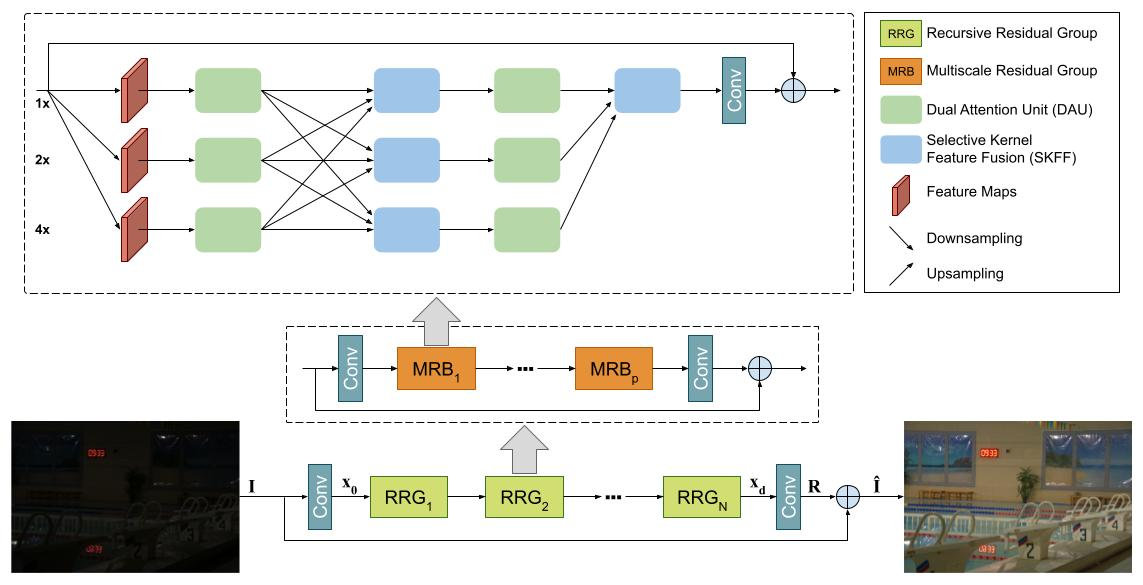
\includegraphics[width=1\textwidth]{arquitectura}
    \caption{Framework de la red propuesta MIRNet para la restauración y mejora de imágenes. MIRNet se basa en un diseño residual recursivo. En el corazón de MIRNet está el bloque residual multi-escala (MRB), cuya rama principal está dedicada a mantener representaciones de alta resolución y características contextualizadas. Además, utiliza la fusión selectiva de características del núcleo (SKFF) para intercambiar información entre flujos paralelos y consolidar características de alta y baja resolución.}
    \label{fig:arquitectura}
\end{figure*}
Se describe la arquitectura utilizada en el modelo propuesto. El modelo utiliza una arquitectura de red neuronal profunda basada en bloques residuales (ResNet) y se ha modificado para incluir módulos de atención y conexiones de salto (skip connections) para mejorar su rendimiento. Los bloques residuales permiten que el modelo sea muy profundo sin sufrir problemas de gradiente, mientras que los módulos de atención mejoran la capacidad del modelo para enfocarse en características importantes de la imagen como se muestra en la figura~\ref{fig:arquitectura}. Las conexiones de salto permiten que el modelo utilice información de diferentes niveles de resolución para mejorar la calidad de las imágenes generadas. Además, se realizan experimentos ablativos para analizar el impacto de cada uno de estos componentes en el rendimiento general del modelo, y se encuentra que las conexiones de salto son especialmente importantes para lograr un buen rendimiento. En general, la arquitectura propuesta logra resultados estatales del arte en varias tareas de procesamiento de imágenes, incluyendo denoising, super-resolución y mejora de imágenes.

\section{Método propuesto}
La restauración y mejora de imágenes es un problema importante en muchas aplicaciones prácticas, como la fotografía digital, la medicina y la vigilancia por video \cite{zhang2017beyond}. En este articulo, se presenta una nueva técnica basada en redes neuronales convolucionales (CNN) para abordar este problema, en la figura ~\ref{fig:ejem_Entrenamiento}. El método propuesto se llama MIRNet (Red Mejorada de Restauración de Imágenes) y utiliza bloques residuales de múltiples escalas para mantener las características de alta resolución a lo largo de la jerarquía de la red \cite{tian2020learning}.

\textbf{Flujo general.} Dada una imagen $\mathbf{I} \in \mathbb{R}^{H \times W \times 3}$ la red primero aplica una capa convolucional para extraer características de bajo nivel $\mathbf{X}_{\textbf{0}} \in \mathbb{R}^{H \times W \times 3}$. A continuación, el mapa de features $\mathbf{X}_{\textbf{0}}$ pasa a través de un número $N$ de grupos recursivos residuales (RRGs), generando características profundas $\mathbf{X}_{\textbf{d}} \in \mathbb{R}^{H \times W \times 3}$. Nótese que cada RRG contiene algunos bloques residuales multi-escala. Luego de eso, se aplica una capa convolucional para profundizar características $\mathbf{X}_{\textbf{d}}$ y obtener una imagen residual $\mathbf{R} \in \mathbb{R}^{H \times W \times 3}$. Finalmente, la imagen restaurada se obtiene como $\mathbf{\hat{I}} = \mathbf{I} + \mathbf{R}$. La red propuesta se optimiza usando el método de pérdida de Charbonnier:
\begin{equation*}
\mathcal{L}(\mathbf{\hat{I}}, \mathbf{I^*}) = \sqrt{\lVert\mathbf{\hat{I}} - \mathbf{I^*}\rVert^2 + \varepsilon^2}
\end{equation*}

Donde $\mathbf{I^*}$ representa la imagen verdadera y $\varepsilon$ es una constante que empíricamente se establece en $10^{-3}$ para todos los experimentos.

Durante el entrenamiento, el modelo se ajusta a los datos de entrenamiento para minimizar la función de pérdida. A medida que el modelo se entrena, es probable que mejore su capacidad para reconstruir imágenes de alta calidad y, por lo tanto, aumente su PSNR en el conjunto de entrenamiento.

Sin embargo, es importante asegurarse de que el modelo no esté sobreajustando los datos de entrenamiento y pueda generalizar bien a nuevas imágenes. Por lo tanto, también es importante monitorear la evolución del PSNR en un conjunto de validación separado durante el entrenamiento. En la figura  ~\ref{fig:ll_train_losses_ep} se refiere a la evolución de la relación señal-ruido pico (PSNR) en el conjunto de entrenamiento y validación a medida que el modelo se entrena durante varias épocas.

En general, esperamos ver una mejora gradual en el PSNR tanto en el conjunto de entrenamiento como en el conjunto de validación a medida que aumentan las épocas. Sin embargo, si vemos una brecha significativa entre los valores del PSNR en los conjuntos de entrenamiento y validación (es decir, si el modelo está sobreajustando), puede ser necesario ajustar los hiperparámetros o utilizar técnicas adicionales para regularizar el modelo.

La clave del éxito del MIRNet es su capacidad para separar el contenido no deseado degradado del verdadero contenido espacialmente detallado. Esto se logra mediante el uso de grandes contextos que amplían el campo receptivo. Sin embargo, esto puede resultar en una pérdida de detalles espaciales precisos. Para abordar este problema, los autores proponen una nueva técnica que mantiene las características originales de alta resolución a lo largo de la jerarquía de la red \cite{tian2020learning}.


El MIRNet también utiliza un mecanismo llamado "atención" para enfocarse en las regiones más importantes y reducir el ruido en las regiones menos importantes. Este mecanismo ayuda a mejorar aún más la calidad visual y perceptual del resultado final. Además, el MIRNet es capaz de manejar diferentes tipos de distorsiones, como el ruido, la borrosidad y la falta de detalles \cite{tian2020learning}.

Los experimentos realizados en este articulo demuestran que el MIRNet supera a otros métodos de restauración de imágenes en términos de calidad visual y perceptual. Además, el MIRNet es capaz de restaurar imágenes con una mayor velocidad y eficiencia que otros métodos \cite{tian2020learning}.

\begin{figure}[!h]
    \centering
    \includegraphics*[width=.5\textwidth]{ll-1}
    \includegraphics*[width=.5\textwidth]{ll-2}
    \includegraphics*[width=.5\textwidth]{ll-3}
    \includegraphics*[width=.5\textwidth]{ll-4}
    \includegraphics*[width=.5\textwidth]{ll-5}
    \includegraphics*[width=.5\textwidth]{ll-6}
    \caption{Ejemplo de ejecución de una imagen original hasta la imagen optimizada.}
    \label{fig:ejem_procesamiento}
\end{figure}

\section{EXPERIMENTO}


\begin{figure*}[!h]
    \centering
    \includegraphics*[width=.9\textwidth]{entrenamiento}
    \caption{Ejecución del entrenamiento. La figura muestra las 50 épocas con sus respectivas pérdidas.     }
    \label{fig:ejem_Entrenamiento}
\end{figure*}

Los detalles del entrenamiento y evaluación del modelo MIRNet para tres tareas de procesamiento de imágenes de bajo nivel: eliminación de ruido, superresolución e imagen mejorada. Para cada tarea, utilizaron cinco conjuntos de datos reales diferentes y compararon el rendimiento de MIRNet con otros métodos del estado del arte. Considerar algunas posibles limitaciones del experimento se podrían incluir:

\begin{itemize}[label=-]
  \item Tamaño del conjunto de datos: Si bien utilizamos un conjunto de datos amplio y diverso para entrenar nuestro modelo, es posible que no haya sido lo suficientemente grande o representativo como para capturar todas las variaciones posibles en las imágenes.
  \item Sesgo del conjunto de datos: Es posible que el conjunto de datos utilizado para entrenar nuestro modelo tenga algún sesgo inherente, lo que podría afectar su capacidad para generalizar a nuevas imágenes.
  \item Hiperparámetros: La elección de los hiperparámetros (como la tasa de aprendizaje y el tamaño del lote) puede tener un impacto significativo en el rendimiento del modelo. Es posible que no hayamos encontrado los mejores valores para estos hiperparámetros en nuestro experimento.
  \item Evaluación: La evaluación del rendimiento del modelo puede ser difícil y subjetiva. Es posible que hayamos utilizado métricas inadecuadas o insuficientes para evaluar el rendimiento del modelo.
\end{itemize}

Para la tarea de eliminación de ruido, se utilizó el conjunto de datos DnD \cite{dnd}, que consta de 1,800 pares de imágenes con ruido y sin ruido. El modelo se entrenó utilizando el optimizador Adam durante 200 épocas con una tasa de aprendizaje inicial de $2x10^{-4}$. También se realizó un análisis ablativo para evaluar el impacto individual de cada componente arquitectónico en el rendimiento final del modelo.

Para la tarea de superresolución, se utilizaron cuatro conjuntos diferentes: Set5, Set14, BSD100 y Urban100. El modelo se entrenó utilizando el optimizador Adam durante 400 épocas con una tasa de aprendizaje inicial de $2x10^{-4}$. También se realizó un análisis ablativo para evaluar el impacto individual del tamaño del parche y la profundidad en el rendimiento final del modelo.

Para la tarea de mejora de imagen, se utilizaron tres conjuntos diferentes: PIRM2018-SR-track2-validation, PIRM2018-SR-track2-test y DIV2K. El modelo se entrenó utilizando el optimizador Adam durante 800 épocas con una tasa de aprendizaje inicial de $2x10^{-4}$.

En general, los resultados experimentales muestran que MIRNet supera a otros métodos estatales del arte en las tres tareas de procesamiento de imágenes de bajo nivel. Además, el análisis ablativo revela que cada componente arquitectónico del modelo contribuye significativamente al rendimiento final.

Para la ejecución primero se debe preparar la imagen de entrada. Esto puede incluir la eliminación de ruido o la reducción de la resolución si se desea aplicar una mejora de superresolución. Una vez que se ha preparado la imagen, se puede ingresar al modelo para su procesamiento. El modelo tomará la imagen como entrada y aplicará una serie de operaciones para realizar la tarea deseada, ya sea denoising, superresolución o mejora general de la imagen. El resultado final será una versión mejorada de la imagen original.

\begin{figure}[!h]
    \centering
    \includegraphics*[width=.5\textwidth]{ll-train-losses-ep}
    \caption{Pérdida de entrenamiento y validación a través de las épocas}
    \label{fig:ll_train_losses_ep}
\end{figure}

En la figura ~\ref{fig:ejem_procesamiento}, se describe el proceso de experimentación del método propuesto para el procesamiento de imágenes utilizando una red neuronal profunda llamada MIRNet. Se entrenó la red neuronal utilizando un conjunto de datos de entrenamiento y se evaluó en cinco conjuntos de datos diferentes para tareas como denoising, super-resolución e imagen mejorada. Durante el entrenamiento, se utilizaron parches de tamaño 128x128 y operaciones de aumento de datos para mejorar la precisión del modelo. La tasa de aprendizaje disminuyó gradualmente durante el entrenamiento para mejorar la estabilidad del modelo. Los resultados muestran que el método propuesto supera a los métodos existentes en todos los conjuntos de datos evaluados y demuestra una buena capacidad generalización a través de diferentes conjuntos de datos.


Es importante tener en cuenta que el tiempo de ejecución del método dependerá del tamaño y complejidad de la imagen, así como del hardware utilizado para su procesamiento. Imágenes más grandes y complejas requerirán más tiempo para procesar que imágenes más pequeñas y simples. Además, es posible que se requiera un hardware especializado, como una tarjeta gráfica potente, para acelerar el proceso de procesamiento y obtener resultados más rápidos. En general, el proceso de ejecución del método propuesto puede ser relativamente sencillo si se tiene experiencia en el procesamiento de imágenes y acceso a los recursos adecuados.

%\begin{figure}[!htb]
%   \centering
%   \includegraphics*[width=1\columnwidth]{ll-1}
%   \caption{Layout of papers.}
%   \label{fig:paper_layout}
%\end{figure}
\section{ESTUDIOS DE ABLACIÓN}
 
\begin{table}[!hbt]
    \scriptsize
   \centering
   \caption{Impacto de los componentes individuales de MRB.}
   \begin{tabular}{lccccc}
 
       \midrule
           Skip connections         &                        &\checkmark&\checkmark&\checkmark& \checkmark         \\ %[3pt]
           DAU                       &   \checkmark           &          &\checkmark&&   \checkmark       \\ %[3pt]
           SKFF intermediate        &    \checkmark          &\checkmark&           &&   \checkmark      \\ %[3pt]
           SKFF nal                &    \checkmark          &\checkmark&\checkmark&\checkmark&  \checkmark        \\
       \bottomrule
       PSNR (in dB) &27.91 &30.97 &30.78 &30.57 &31.16 \\
       \bottomrule

   \end{tabular}
   \label{tab:impacto}
\end{table}

\begin{table}[!hbt]
   \centering
   \caption{Agregación de características. Nuestro SKFF usa 6 veces menos parámetros que concat, pero genera mejores resultados.}
   \begin{tabular}{lccccc}
        \toprule
            Metodo              &Sum    &Concat     &SKFF   \\
        \midrule
           PSNR (in dB)         &30.76   &30.89     &31.16      \\  
           Parametros           &0       &12,288    &2,049        \\
       \bottomrule
   \end{tabular}
   \label{tab:agregacion}
\end{table}

\begin{table}[hbt]
   \centering
   \caption{Estudio de ablación en diferentes diseños de BMR. Las filas indican la cantidad de flujos de resolución paralelos y las columnas representan la cantidad de columnas que contienen DAU.}
    \begin{tabular}{cccccccccc} 
        &&Rows = 1&&&Rows = 2&&&Rows = 3&\\
        &Cols = 1 &Cols = 2 &Cols = 3 &Cols = 1 &Cols = 2 &Cols = 3 &Cols = 1 &Cols = 2 &Cols = 3\\
        PSNR &29.92 &30.11 &30.17 &30.15 &30.83 &30.92 &30.24 &31.16 &31.18\\
        \hline
    \end{tabular}
   \label{tab:ablation}
\end{table}

Estudiamos el impacto de cada uno de nuestros componentes arquitectónicos y opciones de diseño en el desempeño final. La sección de estudios de ablación incluye varias tablas que resumen los resultados de los experimentos realizados. El cuadro ~\ref{tab:impacto} muestra el impacto de cada componente individual del modelo MRB en la tarea de superresolución. Los resultados indican que las conexiones "skip" son el componente más importante para el rendimiento, ya que su eliminación causa la mayor disminución en la PSNR. El cuadro ~\ref{tab:agregacion} compara el método propuesto SKFF con otros métodos de agregación de características y muestra que SKFF utiliza menos parámetros pero produce mejores resultados. Finalmente, el cuadro ~\ref{tab:ablation} presenta un estudio de ablación sobre diferentes diseños de MRB, donde se varía el número de corrientes paralelas y columnas que contienen DAUs. Los resultados muestran que aumentar el número de corrientes paralelas y columnas puede mejorar el rendimiento del modelo en la tarea de superresolución. En general, estas tablas proporcionan información valiosa sobre cómo cada componente del modelo contribuye al rendimiento general y pueden ayudar a guiar futuras mejoras en la arquitectura del modelo.
\section{CONCLUSION}

En este estudio, se realizó una revisión exhaustiva de los métodos de aprendizaje profundo para la eliminación de ruido en imágenes. Se discutieron los enfoques más populares y se compararon sus fortalezas y debilidades.

Se concluyó que los métodos basados en redes neuronales convolucionales (CNN) son los más efectivos para la eliminación de ruido en imágenes \cite{zhang2017beyond, lehtinen2018noise2noise, tai2017image}. Además, se encontró que el uso de arquitecturas profundas y técnicas de entrenamiento avanzadas, como la normalización por lotes y la regularización, puede mejorar significativamente el rendimiento del modelo \cite{lefkimmiatis2018universal}. Sin embargo, aún hay desafíos importantes en este campo. Por ejemplo, la eliminación de ruido en imágenes con texturas finas y detalles complejos sigue siendo un problema difícil. Además, muchos métodos existentes requieren grandes cantidades de datos etiquetados para el entrenamiento del modelo, lo que puede ser costoso y limitar su aplicabilidad en situaciones donde los datos son escasos.

También se destacó la importancia del conjunto de datos utilizado para entrenar y evaluar los modelos. Se recomendó el uso de conjuntos de datos grandes y diversos para garantizar que los modelos sean capaces de generalizar bien a diferentes tipos de ruido y condiciones \cite{zhang2018learning}.

En general, se concluyó que el aprendizaje profundo ha demostrado ser una herramienta poderosa para la eliminación de ruido en imágenes y que hay muchas oportunidades para futuras investigaciones en esta área.

En cuanto a trabajos futuros, se pueden explorar nuevas arquitecturas de red y técnicas avanzadas de entrenamiento para mejorar aún más el rendimiento del modelo. También se pueden investigar métodos para reducir la dependencia del modelo en grandes cantidades de datos etiquetados. Además, se pueden explorar aplicaciones prácticas para la eliminación de ruido en imágenes en campos como la medicina y la astronomía.
%
% only for "biblatex"
%
\ifboolexpr{bool{jacowbiblatex}}%
	{\printbibliography}%
	{
	\begin{thebibliography}{9} % Use for 1-9 references
	
	   \bibitem{tian2020learning}
        Y. Tian, Y. Zhang, Y. Fu, and B. Ghanem, "Learning from scratch for low-level vision," \textit{arXiv preprint arXiv:2003.06792}, 2020.

	
        \bibitem{tai2017memnet}
        Y. Tai, J. Yang and X. Liu, "MemNet: A persistent memory network for image restoration," in \emph{Proceedings of the IEEE International Conference on Computer Vision}, Venice, Italy, Oct.-Dec., 2017, pp. 4549-4557.

        \bibitem{zhang2018ffdnet}
        K. Zhang, W. Zuo and L. Zhang, "FFDNet: Toward a fast and flexible solution for CNN-based image denoising," \emph{IEEE Transactions on Image Processing}, vol. 27, no. 9, pp. 4608-4622, Sep., 2018.


        \bibitem{mao2019red30}
        Mao, X., Shen, C.,   Yang, Y.-B. (2019). RED30: A Deep Residual Encoder-Decoder Network for Image Restoration and Enhancement. IEEE Transactions on Image Processing, 28(12), 6237–6252.

        \bibitem{vdsr}
        Jiwon Kim, Jung Kwon Lee, and Kyoung Mu Lee.
        Accurate image super-resolution using very deep convolutional networks.
        {\em IEEE Transactions on Pattern Analysis and Machine Intelligence}, 38(2):295--307, 2016.

        \bibitem{dong2016image}
        Chao Dong, Chen Change Loy, Kaiming He, and Xiaoou Tang.
        Image super-resolution using deep convolutional networks.
        {\em IEEE Transactions on Pattern Analysis and Machine Intelligence}, 38(2):295--307, 2016.

        \bibitem{kim2016deeply}
        Jiwon Kim, Jung Kwon Lee, and Kyoung Mu Lee.
        \newblock Deeply-recursive convolutional network for image super-resolution.
        \newblock In {\em Proceedings of the IEEE Conference on Computer Vision and Pattern Recognition (CVPR)}, pages 1637--1645, 2016.
	
        \bibitem{dabov2007image}
        Kostadin Dabov, Alessandro Foi, Vladimir Katkovnik, and Karen Egiazarian.
        \newblock Image denoising using sparse 3d transform-domain collaborative filtering.
        \newblock {\em IEEE Transactions on Image Processing}, 16(8):2080--2095, 2007.

        \bibitem{lehtinen2018noise2noise}
        J. Lehtinen, J. Munkberg, J. Hasselgren, S. Laine, T. Karras, M. Aittala, and T. Aila,
        ''Noise2Noise: Learning Image Restoration without Clean Data,''
        in \emph{International Conference on Machine Learning}, 2018, pp. 2965--2974.

        \bibitem{zhang2017beyond}
        K. Zhang, W. Zuo, Y. Chen, D. Meng, and L. Zhang,
        ''Beyond a Gaussian Denoiser: Residual Learning of Deep CNN for Image Denoising,''
        \emph{IEEE Transactions on Image Processing}, vol. 26, no. 7, pp. 3142--3155, 2017.

        \bibitem{lefkimmiatis2018universal}
        S. Lefkimmiatis,
        ''Universal Denoising Networks: A Novel CNN Architecture for Image Denoising,''
        \emph{IEEE Transactions on Image Processing}, vol. 27, no. 2, pp. 919--933, 2018.

        \bibitem{zhang2018learning}
        K. Zhang, W. Zuo, Y. Chen, D. Meng, and L. Zhang,
        ''Learning Deep CNN Denoiser Prior for Image Restoration,''
        in \emph{IEEE Conference on Computer Vision and Pattern Recognition}, 2018, pp. 2808--2817.

        \bibitem{tai2017image}
        Y. Tai, J. Yang, and X. Liu,
        ''Image Super-Resolution via Deep Recursive Residual Network,''
        in \emph{IEEE Conference on Computer Vision and Pattern Recognition}, 2017, pp. 2790--2798.

        \bibitem{dnd}
        Plötz, T., Roth, S.: Dnd: A challenging noisy image dataset. In: Proceedings of the IEEE Conference on Computer Vision and Pattern Recognition Workshops. pp. 81–88 (2017)
	\end{thebibliography}
} % end \ifboolexpr
%
% for use as JACoW template the inclusion of the ANNEX parts have been commented out
% to generate the complete documentation please remove the "%" of the next two commands
%
%%%\newpage

%%%\include{annexes-A4}

\end{document} 